\subsubsection{UC11 - Gestione prenotazioni}
\begin{itemize}
	\item \textbf{Attori Primari}: utente autenticato;
	\item \textbf{Descrizione}: agli utenti autenticati è resa disponibile una maschera che presenta la lista di tutte le sue prenotazioni ancora attive, dalla quale l'utente può scegliere di effettuare operazioni di gestione su ognuna di esse;
	per ogni prenotazione presente nella lista saranno visualizzati dei dettagli riassuntivi, che sono:
	\begin{itemize}
		\item nome del proprietario del veicolo o dell'usufruente
		\item data;
		\item fascia oraria;
		\item marca del veicolo prenotato;
		\item modello del veicolo prenotato;
		\item anno d'immatricolazione del veicolo prenotato.
	\end{itemize}
	\item \textbf{Scenario principale}: l'utente effettua operazioni di gestione di una prenotazione. Esse comprendono:
	\begin{itemize}
		\item visualizzazione dettagli prenotazione [UC11.1];
		\item cancellazione prenotazione [UC11.2].
	\end{itemize}
	\item \textbf{Precondizione}: il sistema carica correttamente la lista di prenotazione effettuate attualmente attive;
	\item \textbf{Post-condizione}: l'utente ha visualizzato le sue prenotazioni correnti ed è riuscito ad effettuare eventuali modifiche.
\end{itemize} 
\begin{figure}[h]
	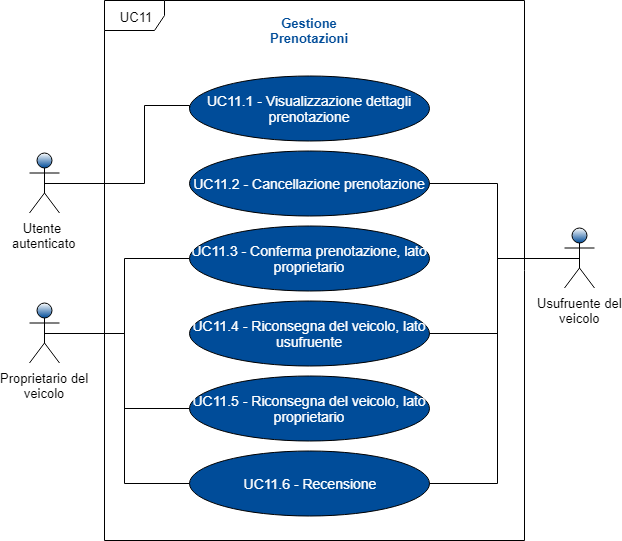
\includegraphics[width=10cm]{res/images/UC11Prenotazione.png}
	\centering
	\caption{UC11 - Gestione prenotazione}
\end{figure}
 \subsubsection{UC11.1 - Visualizzazione dettagli prenotazione}
\begin{itemize}
	\item \textbf{Attori Primari}: utente autenticato;
	\item \textbf{Descrizione}: l'utente visualizza i dettagli della prenotazione scelta dalla maschera di presentazione delle prenotazioni, ciò gli permette di visualizzare:
	\begin{itemize}
		\item la data;
		\item la fascia oraria;
		\item il veicolo prenotato;
		\item il luogo d'incontro con l'altro utente;
		\item l'orario d'incontro;
	\end{itemize}
	\item \textbf{Scenario principale}:
	\begin{itemize}
		\item l'utente sta visualizzando i dettagli della prenotazione;
		\item l'utente sceglie di eliminare la prenotazione scelta [UC11.2];
		\item l'utente riconsegna il veicolo [UC11.3].
	\end{itemize}
	\item \textbf{Precondizione}: l'utente sta visualizzando i dettagli della prenotazione scelta dalla maschera di presentazione delle prenotazioni;
	\item \textbf{Post-condizione}: l'utente ha visualizzato la prenotazione precedentemente scelta.
\end{itemize}
\begin{comment}

\subsubsection{UC6.2 - Modifica di una prenotazione}
\begin{itemize}
	\item \textbf{Attori Primari}: utente autenticato;
	\item \textbf{Descrizione}: l'utente modifica uno o più dati della prenotazione selezionata;
	\item \textbf{Scenario principale}: l'utente si trova all'interno della pagina di modifica della prenotazione precedentemente selezionata;
	\item \textbf{Precondizione}: l'utente si trova nella pagina di presentazione di tutte le sue prenotazioni e ne ha selezionato una per la modifica, oppure l'utente si trova nella pagina di visualizzazione dettagli prenotazione e sceglie di modificare quest'ultima;
	\item \textbf{Post-condizione}: l'utente ha modificato uno o più dati della prenotazione selezionata.
\end{itemize}

\end{comment}
\subsubsection{UC11.2 - Cancellazione prenotazione}
\begin{itemize}
	\item \textbf{Attori Primari}: utente autenticato;
	\item \textbf{Descrizione}: l'utente cancella la prenotazione selezionata;
	\item \textbf{Scenario principale}: l'utente si trova all'interno della pagina di visualizzazione dei dettagli della prenotazione precedentemente selezionata. Attraverso l'apposito pulsante l'utente chiederà la cancellazione della prenotazione;
	\item \textbf{Precondizione}: l'utente visualizza correttamente la prenotazione che intende cancellare;
	\item \textbf{Post-condizione}: l'utente ha annullato correttamente la prenotazione selezionata.
\end{itemize}

\subsubsection{UC11.3 - Riconsegna veicolo}
\begin{itemize}
	\item \textbf{Attori Primari}: utente autenticato;
	\item \textbf{Descrizione}: l'utente riconsegna il veicolo e chiude la prenotazione;
	\item \textbf{Scenario principale}: l'utente si trova all'interno della pagina di visualizzazione dei dettagli della prenotazione precedentemente selezionata. Dopo aver riconsegnato il veicolo e le chiavi, attraverso l'apposito pulsante l'utente chiederà la chiusura della prenotazione. Comparirà un pop-up che permetterà di lasciare una recensione all'altro utente [UC11.4];
	\item \textbf{Precondizione}: l'utente visualizza correttamente la prenotazione che intende concludere;
	\item \textbf{Post-condizione}: l'utente ha concluso correttamente la prenotazione selezionata.
\end{itemize}

\subsubsection{UC11.4 - Recensione}
\begin{itemize}
	\item \textbf{Attori Primari}: utente autenticato;
	\item \textbf{Descrizione}: l'utente recensisce l'altro utente coinvolto nella prenotazione;
	\item \textbf{Scenario principale}: l'utente visualizza il pop-up per inserire la recensione che consiste in una valutazione da una a cinque stelle;
	\item \textbf{Precondizione}: l'utente visualizza correttamente il pop-up;
	\item \textbf{Post-condizione}: l'utente ha inserito correttamente la recensione.
\end{itemize}

